\documentclass[a4paper,14pt]{article}

\usepackage{comment} % Para comentar várias linhas ao mesmo tempo

%matemática
\usepackage{amsmath}
\usepackage{amssymb}

%diagramação
\usepackage{extsizes}
\everymath{\displaystyle}
\usepackage{geometry}
\usepackage{fancyhdr}
\usepackage{multicol}
\usepackage{graphicx}
\usepackage[brazil]{babel}
\usepackage[shortlabels]{enumitem}
\usepackage{cancel}
\usepackage{textcomp}
\usepackage{tcolorbox}

%tabelas
\usepackage{array} % Para melhor formatação de tabelas
\usepackage{longtable}
\usepackage{booktabs}  % Para linhas horizontais mais bonitas
\usepackage{float}   % Para usar o modificador [H]
\usepackage{caption} % Para usar legendas em tabelas
\usepackage{wrapfig} % Para usar tabelas e figuras flutuantes
\usepackage{xcolor} % Para cores do fundo de tabelas
\usepackage{colortbl} % Para cores do fundo de tabelas

%tikzpicture
\begin{comment}
	\usepackage{tikz}
	\usepackage{scalerel}
	\usepackage{pict2e}
	\usepackage{tkz-euclide}
	\usetikzlibrary{calc}
	\usetikzlibrary{patterns,arrows.meta}
	\usetikzlibrary{shadows}
	\usetikzlibrary{external}
\end{comment}


%pgfplots
\usepackage{pgfplots}
\pgfplotsset{compat=newest}
\usepgfplotslibrary{statistics}
\usepgfplotslibrary{fillbetween}

%colours
\usepackage{xcolor}



\columnsep=2cm
\hoffset=0cm
\textwidth=8cm
\setlength{\columnseprule}{.1pt}
\setlength{\columnsep}{2cm}
\renewcommand{\headrulewidth}{0pt}
\geometry{top=1in, bottom=1in, left=0.7in, right=0.5in}

\pagestyle{fancy}
\fancyhf{}
\fancyfoot[C]{\thepage}

\begin{document}
	
	\noindent\textbf{6FMA20 - Matemática} 
	
	\begin{center}Conjunto dos inteiros e sua representação na reta (Versão estudante)
	\end{center}
	
	\noindent\textbf{Nome:} \underline{\hspace{10cm}}
	\noindent\textbf{Data:} \underline{\hspace{4cm}}
	
	%\section*{Questões de Matemática}
	
	\begin{multicols}{2}
		\noindent O conjunto dos números inteiros é representado pela letra $\mathbb{Z}$, escolhemos um sentido em uma reta, ou seja, se os números positivos ficam à direita ou à esquerda do zero. O mais usual é utilizar uma reta horizontal e o sentido da esquerda para a direita, isto é, os números positivos ficam à direita do zero, e os negativos, à esquerda. \\
		Existem outras orientações na reta para representar $\mathbb{Z}$. Para utilizá-las, basta deixarmos claro qual sentido escolhemos. \\
		\noindent\textsubscript{-----------------------------------------------------------------------}
		\begin{enumerate} 
			\item Desenhe uma reta onde você possa colocar os números 0, -1, -2, -3, -4, 1, 2, 3, 4 e outros, se você quiser, sendo que:
			\begin{enumerate}[a)]
				\item a reta seja horizontal e o sentido seja da esquerda para a direita. \\\\\\\\\\
				\item a reta seja horizontal e o sentido seja da direita para a esquerda. \\\\\\\\\\
				\item a reta seja vertical e o sentido seja de baixo para cima. \\\\\\\\\\\\\\\\\\
				\item a reta seja vertical e o sentido seja de cima para baixo. \\\\\\\\\\\\\\\\\\
				\item a reta tenha uma direção que não seja horizontal nem vertical. Indicar nesse caso o sentido da reta. \\\\\\\\\\\\\\\\\\
			\end{enumerate}	
			%71 e 72
			\item Desenhe uma reta horizontal e uma vertical cujos sentidos sejam para a direita e para baixo, respectivamente, e represente os números 0, -5, 5, -3, 3, -8 e 8. \\\\\\\\\\\\\\\\\\\\\\
			\item Veja as ilustrações e escreva quanto vale $x$ e $-x$. \\
			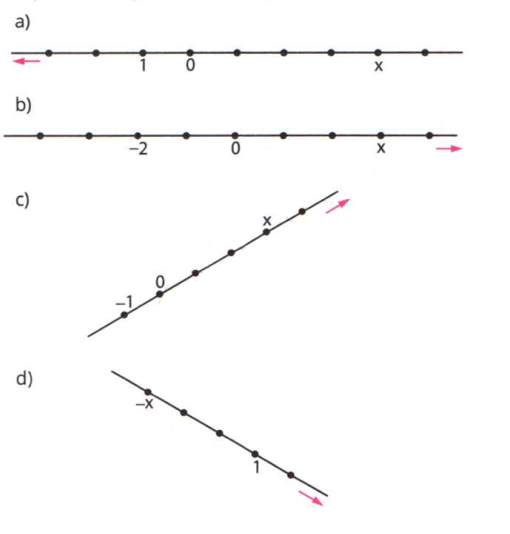
\includegraphics[width=1.2\linewidth]{6FMA20_imagens/imagem1}
		\end{enumerate}
		$~$ \\ $~$ \\ $~$ \\ $~$ \\ $~$ \\ $~$ \\ $~$ \\ $~$ \\ $~$ \\ $~$ \\ $~$ \\ $~$ \\ $~$ \\ $~$ \\ $~$ \\ $~$ \\ $~$ \\ $~$ \\ $~$ \\ $~$ \\ $~$ \\ $~$ \\ $~$ \\ $~$ \\ $~$ \\ $~$ \\ $~$ \\ $~$ \\ $~$ \\ $~$ \\ $~$ \\ $~$ \\ $~$ \\ $~$ \\ $~$ \\ $~$ \\ $~$ \\ $~$ \\ $~$ \\ $~$ \\ $~$ \\ $~$ \\ $~$ \\ $~$ \\ $~$ \\ $~$ \\ $~$ \\ $~$ \\ $~$
	\end{multicols}
\end{document}